\section{Iteratoren}


\subsection{Grundlegendes}

\begin{frame}[fragile]{Grundlegendes}
	\begin{itemize}
		\item Einheitlicher Zugriff auf alle STL-Container
		\item Dadurch Algorithmen leicht auf unterschiedliche Container anzuwenden
		\item Notwendig für Container ohne Random Access (list)
		\item Praktisch für Assoziative container (set, map)
		\item Verallgemeinerung von Pointern
	\end{itemize}
\end{frame}

\begin{frame}[fragile]{Beispiel anhand \texttt{list}}
	\begin{lstlisting}[]
#include <list>
using intList = std::list<int>;
using intIt = intList::iterator;
intList meineListe;
meineListe.push_back(42);
meineListe.push_back(1024);
meineListe.push_front(1);

// C++03
for(intIt it  = meineListe.begin();
          it != meineListe.end();
        ++it) {
    std::cout << *it << std::endl;
}
// C++11
for(int i : meineListe) {
    std::cout << i << std::endl;
}
	\end{lstlisting}
\end{frame}

\begin{frame}[fragile]{\texttt{begin} und \texttt{end}}
	\begin{itemize}
		\item jeder STL-Container hat member functions \texttt{begin} und \texttt{end}
		\item Adapter nicht unbedingt (wo es eben keinen Sinn ergibt\dots)
		\item \texttt{std::begin} in \texttt{<iterator>} für alle Container und plain-C-Arrays
		\item \texttt{begin} liefert einen Iterator, der auf das erste Element zeigt
		\item \texttt{end} liefert einen speziellen Iterator, der sozusagen auf das (letztes~+~1)ste Element zeigt
		\item man iteriert über $[\texttt{begin}, \texttt{end})$, ebenso arbeiten Algorithmen alle auf einem $[x, y)$-Bereich
	\end{itemize}
	
	\pause
	\vspace{1em}
	
	Nützlich: backwards-compatible zu Pointern:
	\begin{lstlisting}
		char const myString[] = "foobar";
		char const* myStringEnd = (myString+5) + 1;
		using It = char const*;
		
		for(It i = myString; i != myStringEnd; ++i)
		{ std::cout << *i; }
	\end{lstlisting}
\end{frame}


\subsection{Iteratoren und Generizität}

\begin{frame}[t]{generischer Ansatz}
	\onslide*<+> { \lstinputlisting[linerange=begin-main]{cpp-code/iterator-functempl.cpp} }
	\onslide<+-> { \lstinputlisting[linerange=begin-]{cpp-code/iterator-functempl.cpp} }
\end{frame}

\begin{frame}[fragile]{STL und Iteratoren}
	Iteratoren bilden das Bindeglied zwischen Containern und Algorithmen, z.B.:
	\begin{lstlisting}
		std::vector < int > myVec = { 4, 3, 1, 2 };
		std::sort( myVec.begin(), myVec.end() );
	\end{lstlisting}
	
	\pause
	\vspace{2em}
	
	Mittels Iteratoren lassen sich auch Daten überführen:
	\begin{lstlisting}
		std::vector < int > myVec = { 4, 4, 4, 3 };
		std::list < int > myList = {myVec.begin(), myVec.end()};
	\end{lstlisting}
\end{frame}


\subsection{Iterator-Kategorien}

\begin{frame}{Iterator-Kategorien}
	\footnotesize
	
	Inspiration: \url{http://en.cppreference.com/w/cpp/iterator}
	\vspace{0.5em}
	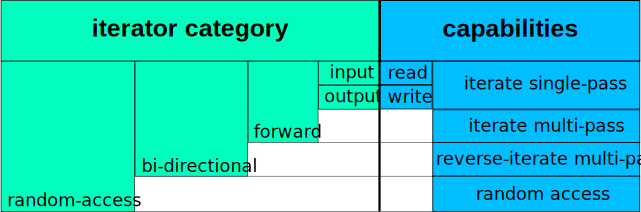
\includegraphics[width=\textwidth]{images/iterator-categories}
	
	\vspace{0.5em}
	\pause
	
	\begin{columns}
		\hspace{13em}
		\column{0.3\textwidth}
			Mit:\\
			\texttt{iterator i, j;}	\\
			\texttt{value\_t value;}	\\
			\texttt{int n;}	\\
			
		\column{0.45\textwidth}
			\begin{tabular}{l|l}
				\textbf{capability}	&	\textbf{syntax}	\\
				\hline
				read	&	\texttt{value = *i}	\\
				write	&	\texttt{*i = value}	\\
				iterate	&	\texttt{++i}, \texttt{i++}	\\
				reverse-iterate	&	\texttt{--i}, \texttt{i--}	\\
				random access &	\texttt{j = i + n}	\\
			\end{tabular}
	\end{columns}
\end{frame}

\begin{frame}{Iterator-Kategorien und Datenstrukturen}
	\begin{center}
		\begin{tabular}{c|c}
			\textbf{Datenstruktur}	&	\textbf{Iterator}	\\
			\hline
			\texttt{vector}	&	random-acccess	\\
			\texttt{list}	&	bi-directional	\\
			\texttt{map}	&	bi-directional	\\
			input stream	&	input	\\
			output stream	&	output	\\
			io stream		&	forward	\\
		\end{tabular}
	\end{center}
\end{frame}
